\documentclass[10pt]{article}

%%%%%%%%%%%%%%%%%%%%%%%%%%%%%%%%%%%%%%%%%%%%%%%%%%%%%%%%%%%%%%%%%%%%%%%%%%%%%%%
%%% packages %%%
%%%%%%%%%%%%%%%%%%%%%%%%%%%%%%%%%%%%%%%%%%%%%%%%%%%%%%%%%%%%%%%%%%%%%%%%%%%%%%%

\usepackage[english]{babel} % Choose english language
\usepackage[labelfont = bf, font = small]{caption} % Use caption package. Use bold font for caption.
\usepackage{siunitx} % Use siunitx for unit representation.
\newcommand{\RM}[1]{\MakeUppercase{\romannumeral #1{:}}}
\usepackage{graphicx}
\usepackage{tabularx}
\usepackage{float}
\usepackage{lmodern}
\usepackage{filecontents}
\usepackage{amsmath}
\usepackage{amssymb}
\usepackage[utf8]{inputenc}
\usepackage[bottom]{footmisc}
\usepackage{leftidx}
\usepackage{subcaption}
\usepackage[explicit]{titlesec}
\usepackage{booktabs}
\usepackage{multirow}
\usepackage{multicol}
\usepackage{listings}
\usepackage{pgfplots}
\usepackage{natbib}
\usepackage{xcolor}
\usepackage{url}
\usepackage{array}
\usepackage{setspace}
\usepackage{hyperref} % Referencing
\usepackage{verbatim}
\usepackage{changepage}
\usepackage[footnote, printonlyused]{acronym}
\usepackage{scrextend}
\usepackage{geometry} % Change geometry of page layout
\usepackage{rotating}
\usepackage{longtable}
\usepackage{lscape}
\usepackage{tocloft}
\usepackage{listings}
\usepackage{feynmp-auto} % Create fenynman diagrams
\usepackage{tikz-feynman} % Create fenynman diagrams
\usepackage{lipsum} % For testing. insert random text

%%%%%%%%%%%%%%%%%%%%%%%%%%%%%%%%%%%%%%%%%%%%%%%%%%%%%%%%%%%%%%%%%%%%%%%%%%%%%%%
%%% new commands and environments %%%
%%%%%%%%%%%%%%%%%%%%%%%%%%%%%%%%%%%%%%%%%%%%%%%%%%%%%%%%%%%%%%%%%%%%%%%%%%%%%%%

% Create custom font
\newenvironment{myfont}{\fontfamily{put}\selectfont}{\par}

% Adapt spacing between lines
\doublespacing

% Delete dots from toc
\renewcommand{\cftdot}{}

% Change section label to roman
\renewcommand{\thesection}{\Roman{section}} 

% Customize section layout
\newcommand{\ssection}[1]{%
  \section[#1]{\centering\normalfont\scshape #1}}
\newcommand{\ssubsection}[1]{%
  \subsection[#1]{\centering\normalfont\itshape #1}}  
\newcommand{\ssubsubsection}[1]{%
  \subsubsection[#1]{\centering\normalfont #1}}

% Import tikz libraries for figures
\usetikzlibrary{positioning,shadows,arrows}

% Create footnotereferencing
\makeatletter
\newcommand\footnoteref[1]{\protected@xdef\@thefnmark{\ref{#1}}\@footnotemark}
\makeatother

% Change layout of page
\hypersetup{
	colorlinks = true,
  linkbordercolor = {red},
  citebordercolor = {red},
  menubordercolor = {blue},
  urlbordercolor = {blue},
  linktoc = {page},
  pagebackref = {True},
  pdftitle = {Solution 01},
  pdfauthor = {Nils Hoyer},
  pdfcreator  = {pdflatex},
  pdfproducer = {LaTeX}
}

% Change geometry of page
\geometry{a4paper, top = 20mm, left = 20mm, right = 20mm, bottom = 15mm, headsep = 8mm, footskip = 10mm, includeheadfoot}

% Decalre uits for SIunitx
\DeclareSIUnit\femtobarn{fb^{-1}}

% Define colors
\definecolor{deepblue}{rgb}{0,0,0.5}
\definecolor{deepred}{rgb}{0.6,0,0}
\definecolor{deepgreen}{rgb}{0,0.6,0.2}
\definecolor{deeporange}{rgb}{0.9,0.2,0}

%%%%%%%%%%%%%%%%%%%%%%%%%%%%%%%%%%%%%%%%%%%%%%%%%%%%%%%%%%%%%%%%%%%%%%%%%%%%%%%
%%% start document %%%
%%%%%%%%%%%%%%%%%%%%%%%%%%%%%%%%%%%%%%%%%%%%%%%%%%%%%%%%%%%%%%%%%%%%%%%%%%%%%%%

\begin{document}
\begin{myfont}
\lstset{language=C++,
  basicstyle=\ttfamily,
  keywordstyle=\color{blue}\ttfamily,
  stringstyle=\color{red}\ttfamily,
  commentstyle=\color{green}\ttfamily,
  morecomment=[l][\color{magenta}]{\#}
}



\begin{center}
	\begin{Large}
		\textsc{Solution for homework assignment no. 02} \\
	\end{Large}
	\vspace*{0.4cm}
		Nils Hoyer, Maurice Morgenthaler
		\vspace*{1cm}
\end{center}

\section*{Exercise 2.1}

We are given a function $f$ which is defined as
\begin{equation}
f(x) =
\begin{cases}
0                           & \textrm{for}\; a \leq x \leq b \\
\frac{2(x-a)}{(b-a)(c-a)}   & \textrm{for}\; a \leq x < c \\
\frac{2(b-x)}{(b-a)(b-c)}   & \textrm{for}\; c \leq x < b \\
\end{cases}
\end{equation}

\noindent and are asked to calculate its mean, mode, median and variance.
We will consider the case where $c = 0$. \\

\noindent Mean $\mu$: $\;\mu = E[x] = \int\limits_{-\infty}^{\infty}dx \cdot xf(x)$ \\
\noindent Median $M$: $\;\frac{1}{2} = \int\limits_{-\infty}^{M}dx \cdot f(x)$ \\
\noindent Mode $m$: $\;\frac{\partial f}{\partial x}(x)|_{x = m} = 0$ \\
\noindent Variance $\sigma^{2}$: $\;\sigma^{2} = E[(x - E[x])^{2}] = \int\limits_{-\infty}^{\infty}dx \cdot (x - \mu)^{2}f(x)$

\begin{itemize}
  \item[\textbf{a)}] For $a = -b$ the function $f(x)$ is defined as
  $$
  f(x) = 
  \begin{cases}
  0                         & \textrm{for}\; x \leq -b \; \textrm{and}\; x \geq b \\
  \frac{x+b}{b^{2}}         & \textrm{for}\; -b \leq x \leq 0 \\
  \frac{b-x}{b^{2}}         & \textrm{for}\; 0 \leq x \leq b \\
  \end{cases}
  $$
  \noindent \textbf{Mean}: Since $f(x)$ and $x$ are odd functions their product is an even function. 
  Since we integrate over a symmetric interval the mean is zero. \\

  \noindent \textbf{Median}: Because of symmerty we know that $M = 0$. \\

  \noindent \textbf{Mode}: Again, due to symmetry and because of the fact that the function is rising for $x \leq 0$ and falling for $x \geq 0$, the mode is zero. \\

  \noindent \textbf{Variance}:
  \begin{align*}
  \sigma^{2} & = \int\limits_{-\infty}^{\infty}dx \cdot (x - \mu)^{2}f(x) = \int\limits_{-b}^{0}dx \cdot x^{2}\frac{x+b}{b^{2}} + \int\limits_{0}^{b}dx \cdot x^{2}\frac{b-x}{b^{2}} \\
             & = \frac{1}{b^{2}}\left[-\frac{b^{4}}{4} + \frac{b^{4}}{3} + \frac{b^{4}}{3} - \frac{b^{4}}{4}\right] = \frac{b^{2}}{6}
  \end{align*}

  \item[\textbf{b)}] For $a = -2b$ the function $f(x)$ is defined as
  $$
  f(x) = 
  \begin{cases}
  0                            & \textrm{for}\; x \leq -2b \; \textrm{and}\; x \geq b \\
  \frac{x+b}{3b^{2}}           & \textrm{for}\; -2b \leq x \leq 0 \\
  \frac{2}{3}\frac{b-x}{b^{2}} & \textrm{for}\; 0 \leq x \leq b \\
  \end{cases}
  $$

  \noindent \textbf{Mean}:
  \begin{align*}
  \mu & = \int\limits_{-\infty}^{\infty}dx \cdot xf(x) = \int\limits_{-2b}^{0}dx \cdot x\frac{x+2b}{3b^{2}} + \int\limits_{0}^{b}dx \cdot x\frac{2}{3}\frac{b-x}{b^{2}} \\
      & = \frac{1}{3b^{2}}\left[\frac{8b^{3}}{3} - 4b^{3} + b^{3} - \frac{2b^{3}}{3}\right] = -\frac{b}{3}
  \end{align*}


  \noindent \textbf{Median}: I suspect that the median lies between $x = -2b$ and $x = 0$.
  \begin{align*}
  \frac{1}{2}         & = \int\limits_{-\infty}^{M}dx \cdot f(x) = \int\limits_{-2b}^{M}dx \cdot \frac{x+2b}{3b^{2}} \\
                      & = \frac{1}{3b^{2}} \left[\frac{M^{2}}{2} + 2bM + 2b^{2}\right] \\
  \Rightarrow M_{1,2} & = -2b \pm \sqrt{3}b
  \end{align*}
  \noindent The only reasonable solution is $M = (-2 + \sqrt{3})b$.

  \noindent \textbf{Mode}: Same argument as before: Since $f_{1}$ (function defined for $x \leq 0$) is rising and $f_{2}$ is falling the mode lies at zero. \\

  \noindent \textbf{Variance}: 
  \begin{align*}
  \sigma^{2} & = \int\limits_{-\infty}^{\infty}dx \cdot (x - \mu)^{2}f(x) = \int\limits_{-2b}^{0}dx \cdot \left(x + \frac{b}{3}\right)^{2}\frac{x+b}{3b^{2}} + \int\limits_{0}^{b}dx \cdot \left(x + \frac{b}{3}\right)^{2}\frac{2(b-x)}{3b^{2}} \\
             & = ... \\
             & = \frac{7}{18}b^{2}
  \end{align*}
\end{itemize}

\section*{Exercise 2.2}

The solution for this quesstion can be found in a file named \texttt{exercise2\_2.C}.


\section*{Exercise 2.3}

You can find the solution for this exercise in a file named \texttt{exercise2\_3.C}.
The resulting plots will be displayed here and attatched to the email.

\begin{figure}[H]
\centering
\caption{This plot summarizes the first two tasks given in this exercise.
On the top left corner is the two dimensional histogram of the distribution of the pion energies.
The other two histograms show the projection on each axis.}
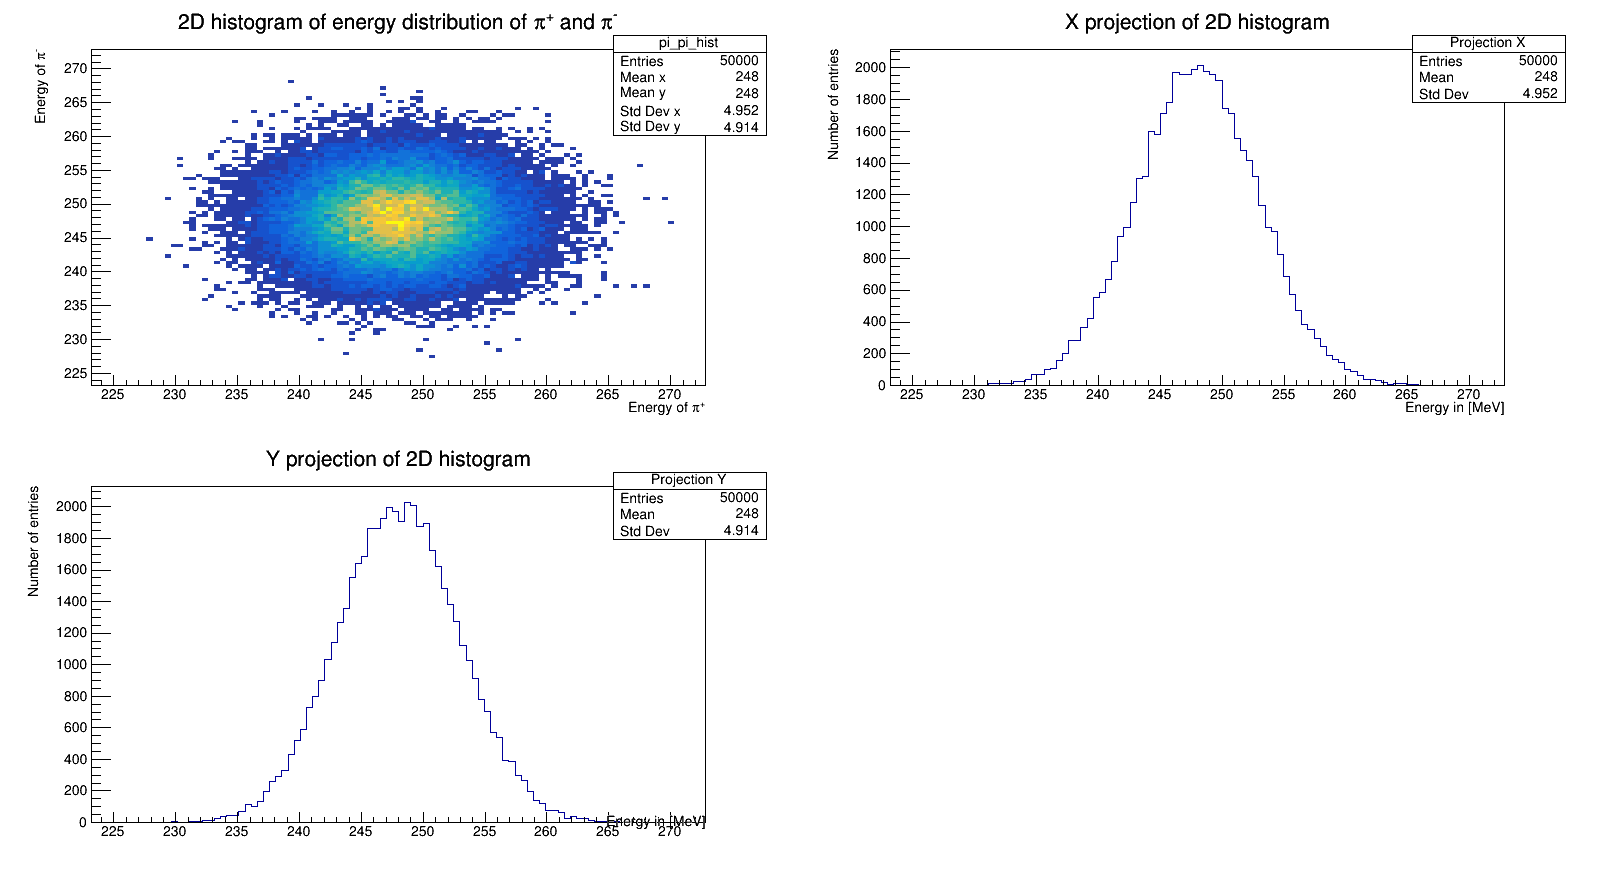
\includegraphics[width = \textwidth]{./canvas.png}
\end{figure}


\begin{figure}[H]
\centering
\caption{This plot summarizes the last task given in this exercise.
The top two histograms show all entries which have a are in bin 50 and 70, respectively.
The bottom histogram shows both individual histograms combined in one graph.}
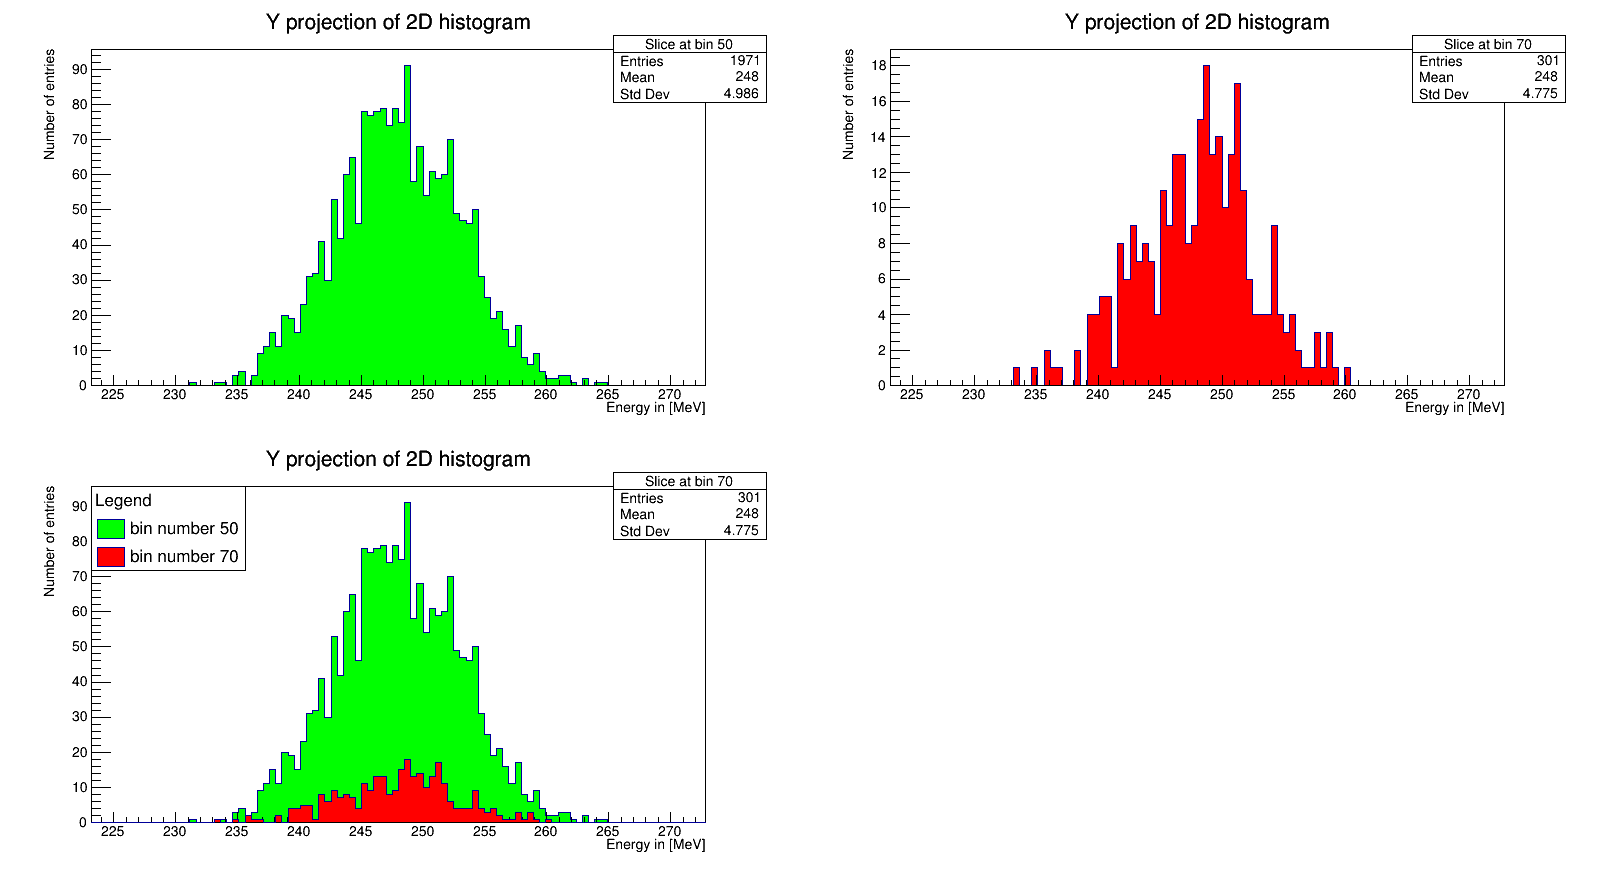
\includegraphics[width = \textwidth]{./canvas2.png}
\end{figure}

\end{myfont}
\end{document}